\section{Forces de frottement de glissement}
    \subsection{Résultante des actions de contact entre deux solides}

        Les actions de contact sont réparties sur la surface de contact. Pour modéliser ces actions, on introduit un modèle qu'est la résultante (ou somme) des actions de contact en un point $I$ de l'interface. Un premier exemple est donné à la Figure~\ref{fig:resultante_1}, où l'équilibre s'écrit $\vec{N}+m\vec{g}=\vec{0}$. Un deuxième exemple est donné à la Figure~\ref{fig:resultante_2} où l'équilibre s'écrit $\vec{N}+m\vec{g}=\vec{0}$ et $\vec{F}+\vec{T}=\vec{0}$.

        Le solide subit donc une résultante $\vec{R}=\vec{N}+\vec{T}$. $\vec{N}$ traduit l'existence de contact, $\vec{T}$ le frottement de glissement. $\vec{T}$ s'oppose au glissement, mais pas au mouvement.

        \begin{figure}
            \centering
            \tikzsetnextfilename{resultante_1}
            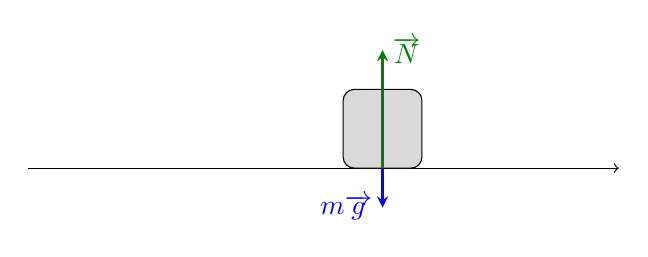
\begin{tikzpicture}[scale=1]  
                % \helpgrid{3}{3}
                \draw [->] (-4.5,-0.5) -- (3,-0.5) ;  
                \coordinate (M) at (0,0);
                \draw[rounded corners=4pt,fill=gray!30] (-0.5,-0.5) rectangle++ (1,1) node [midway, shift=({0,0.05})] {$\centerdot$}; 
                \draw [->,-stealth,thick,blue] (M) --++(0,-1) node [left] {$m\overrightarrow{g}$};   
                \draw [->,-stealth,thick,green!50!black] (M)++(0,-0.5) --++(0,+1.5) node [right] {$\overrightarrow{N}$};   
            \end{tikzpicture}
            \caption{Premier exemple de frottements solides et résultante.}    
            \label{fig:resultante_1}
        \end{figure}

        \begin{figure}
            \centering
            \tikzsetnextfilename{resultante_2}
            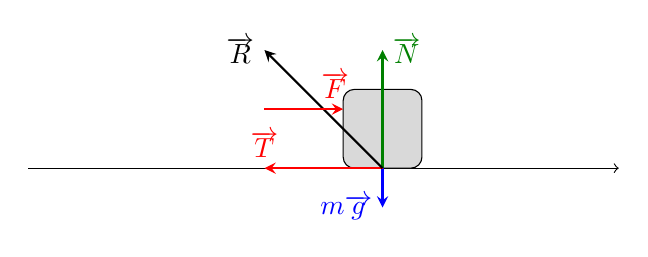
\begin{tikzpicture}[scale=1]  
                % \helpgrid{3}{3}
                \draw [->] (-4.5,-0.5) -- (3,-0.5) ;  
                \coordinate (M) at (0,0);
                \draw[rounded corners=4pt,fill=gray!30] (-0.5,-0.5) rectangle++ (1,1) node [midway, shift=({0,0.05})] {$\centerdot$}; 
                \draw [->,-stealth,thick,blue] (M) --++(0,-1) node [left] {$m\overrightarrow{g}$};   
                \draw [->,-stealth,thick,green!50!black] (M)++(0,-0.5) --++(0,+1.5) node [right] {$\overrightarrow{N}$};   
                \draw [->,-stealth,thick,red] (M)++(0,-0.5)--++(-1.5,0) node [above] {$\overrightarrow{T}$};
                \draw [->,-stealth,thick] (M)++(0,-0.5)--++(-1.5,1.5) node [left] {$\overrightarrow{R}$}; 
                \draw [->,-stealth,thick,red] (-1.5,0.25)--++(1,0) node [above, pos=0.9] {$\overrightarrow{F}$}; 
            \end{tikzpicture}
            \caption{Deuxième exemple de frottements solides et résultante.}    
            \label{fig:resultante_2}
        \end{figure}

    \subsection{Les trois effets possibles des frottements solides}

        On donne différents exemples :
        \begin{enumerate}
            \item la Figure~\ref{fig:effet_frottement_solide_1} décrit un maintien à l'équilibre possible grâce aux frottements.
            \item la Figure~\ref{fig:effet_frottement_solide_2} décrit un premier mouvement gauche-droite où le frottement est responsable du mouvement, c'est une phase de non glissement. Pour le mouvement droite-gauche, la phase de glissement existe à cause de la force de rappel du fil élastique. Les frottements sont responsables d'un freinage.
            \item Lors de la marche à pied, pour se déplacer, il faut une composante tangentielle venant du sol sur les semelles des chaussures.
            \item Les roues des voitures : lors de l'accélération (roues qui patinent), il y a des frottements moteurs, voir la Figure~\ref{fig:effet_frottement_solide_3}. Lors du freinage (roues bloquées), c'est l'inverse.
        \end{enumerate}

        Ainsi, il y a trois effets possibles : maintien à l'équilibre, mise en mouvement et freinage.

        \begin{figure}
            \centering
            \tikzsetnextfilename{effet_frottement_solide_1}
            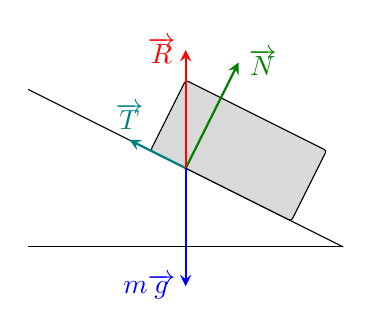
\begin{tikzpicture}[scale=1]  

                \coordinate (O) at (0,0); 
                \coordinate (A) at (-2,1); 
                \draw (O)--++(-4,0);
                \draw (O)--++(-4,2);

                \begin{scope}[rotate=atan((3-0)/(2-8))]
                    \draw  [rounded corners=1pt,fill=gray!30] ([shift={(-0.5,0)}]A) rectangle ++(2,1);
                    \draw [->,-stealth,thick,green!50!black] (A)--++(0,+1.5) node [right] {$\overrightarrow{N}$};
                    \draw [->,-stealth,thick,green!50!blue] (A)--++(-0.8,0) node [above] {$\overrightarrow{T}$};  
                \end{scope}

                \draw [->,-stealth,thick,blue] (A)--++(0,-1.5) node [left] {$m\overrightarrow{g}$};
                \draw [->,-stealth,thick,red] (A)--++(0,1.5) node [left] {$\overrightarrow{R}$};   
            \end{tikzpicture}
            \caption{Premier exemple d'effet possible des frottements solides.}
            \label{fig:effet_frottement_solide_1}
        \end{figure}

        \begin{figure}
            \centering
            \tikzsetnextfilename{effet_frottement_solide_2}
            \begin{tikzpicture}[scale=1]  

            \coordinate (O) at (0,0); 
            \node at (-3.6,0)[below] {O};
            
            \draw [->,-stealth,thick] (-3.6,0.35) -- (1,0.35) node [below]{$z$};
            
            %ressort   
            \begin{scope}[shift=({0,0})]     

            \begin{scope}[scale=0.75,shift=({-4.78,0.5}),rotate around={90:(0,0)}]
            %bloc qui tient le ressort
                \draw[thick,gray] (0,0) -- (0,-0.3); 
                \fill [pattern=north east lines] (-0.5,0) rectangle (0.5,0.3); 
                \draw[thick](-0.5,0)--(0.5,0);
                %fin ressort       
            \end{scope}	

            \draw [ressort,decorate,decoration={coil,aspect=0.6,segment length=5mm,amplitude=3mm}] (-3.375,0.36)--++(3,0) ;
            \draw[rounded corners=1pt,fill=gray!30] (-0.5,0.35) rectangle++ (0.5,0.5) node [midway, shift=({0,0.05})] {$\centerdot$};  

            \draw [->,green!50!black,very thick] (-0.25,0.35)--++(1,0) node [below] {$\overrightarrow{T}$};
            \draw [->,red!50!black,very thick] (-0.25,0.57)--++(0.5,0) node [above] {$\overrightarrow{v}$};
            \end{scope}

        \end{tikzpicture}
        \caption[Deuxième exemple d'effet possible des frottements solides]{Deuxième exemple d'effet possible des frottements solides. L'axe est un tapis roulant vers la droite.}
        \label{fig:effet_frottement_solide_2}
        \end{figure}

        \begin{figure}
            \centering
            \tikzsetnextfilename{effet_frottement_solide_3}
            \begin{tikzpicture}[scale=1]
                %\helpgrid{2}{2};
                
                \draw[
                    decoration={markings, mark=at position 0.625 with {\arrow{<}}},
                    postaction={decorate}
                    ]
                    (0,0) circle (1);
                \draw [->] (0.25,0.75) to [bend left=90] (0.25,-0.75);
                \node at (0.15,0) {$\vec{\omega}$};
                \draw [->,blue!50!black,very thick] (0,-1)--++(2.5,0) node [above] {$\overrightarrow{T}$};
                \draw [->,red!50!black,very thick] (0,-1)--++(-2.5,0) node [above] {$\overrightarrow{v}_g$};
            \end{tikzpicture}
            \caption{Troisième exemple d'effet possible des frottements solides.}
            \label{fig:effet_frottement_solide_3}
        \end{figure}

    \subsection{Lois empiriques de Coulomb--Amontons du frottement solide}

        \paragraph{Notions de vitesse de glissement.}

            \begin{figure}
                \centering
                \tikzsetnextfilename{notion_vitesse_glissement}
                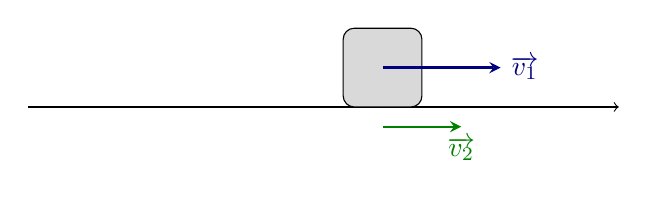
\begin{tikzpicture}[scale=1]  
                    % \helpgrid{3}{3}
                    \draw [->] (-4.5,-0.5) -- (3,-0.5) ;  
                    \coordinate (M) at (0,0);
                    \draw[rounded corners=4pt,fill=gray!30] (-0.5,-0.5) rectangle++ (1,1) node [midway, shift=({0,0.05})] {$\centerdot$}; 
                    \draw [->,-stealth,thick,blue!50!black] (M)--++(1.5,0) node [right] {$\overrightarrow{v_1}$};
                    \draw [->,-stealth,thick,green!50!black] (M)++(0,-0.75) --++(1.,0) node [below] {$\overrightarrow{v_2}$};   
                \end{tikzpicture}
                \caption{Notion de vitesse de glissement.}    
                \label{fig:notion_vitesse_glissement}
            \end{figure}

            La Figure~\ref{fig:notion_vitesse_glissement} présente un solide en mouvement du solide (1) par rapport au sol (2). Alors la vitesse de glissement est définie par 
            \begin{equation*}
                \vec{v}_g(1/2)\coloneqq =\vec{v}_1-\vec{v}_2.
            \end{equation*}

            Il faut noter que cette définition est indépendante du référentiel : si $\mathcal{R}_2$ est un référentiel lié à 2, alors 
            \begin{equation*}
                \vec{v}'_{1/2}-\vec{v}'_{2/\mathcal{R}_2}=\vec{v}_1-\vec{v}_2=\vec{v}_g.
            \end{equation*}

        \paragraph{Cas du glissement.} 
            
            On est donc dans le cas où $\vec{v}_g\neq\vec{0}$. Alors
            \begin{enumerate}
                \item $\vec{T}\parallel\vec{v}_g$ et $\vec{T}\cdot\vec{v}_g<0$ : $\vec{T}$ et $\vec{v}_g$ sont de sens opposés.
                \item On a $\left\lVert\vec{T}\right\rVert=f_d\left\lVert\vec{N}\right\rVert$. $f_g$ est le coefficient de frottement dynamique : il est indépendant de $\left\lVert\vec{N}\right\rVert$ et de la surface de contact, mais dépend de la nature des matériaux et de l'état des surfaces.
            \end{enumerate}

        \paragraph{Cas du non glissement.} 
        
            On est donc dans le cas où $\vec{v}_g=\vec{0}$. Alors on a
            \begin{equation*}
                \left\lVert\vec{T}\right\rVert\leqslant f_s\left\lVert\vec{N}\right\rVert,
            \end{equation*}
            où $f_s$ est le coefficient de frottement statique. $f_s$ et $f_d$ ont les mêmes propriétés et en général, $f_s\geqslant f_d$.


        \paragraph{Cône de frottement.}

            \subparagraph{Non glissement.} Soit $\varphi_{s}$ tel que $f_s=\tan\varphi_s$. Alors 
            \begin{equation*}
                \left\lVert\vec{T}\right\rVert\leqslant f_s\left\lVert\vec{N}\right\rVert\Leftrightarrow\tan(\alpha)\leqslant\tan\varphi_s\Leftrightarrow\alpha\leqslant\varphi_s.
            \end{equation*}
            Il y a non glissement si la résultante $\vec{R}$ reste à l'intérieur du cône de frottement statique, voir la Figure~\ref{fig:cone_frottement_statique}.

            \subparagraph{Glissement.} Soit $\varphi_{d}$ tel que $f_d=\tan\varphi_d$. Alors 
            \begin{equation*}
                \left\lVert\vec{T}\right\rVert= f_d\left\lVert\vec{N}\right\rVert\Leftrightarrow\tan(\alpha)=\tan\varphi_d\Leftrightarrow\alpha=\varphi_d.
            \end{equation*}
            Il y a glissement si la résultante $\vec{R}$ coïncide avec le bord du cône de frottement dynamique, voir la Figure~\ref{fig:cone_frottement_dynamique}.

            \begin{figure}
                \centering
                \tikzsetnextfilename{cone_frottement_statique}
                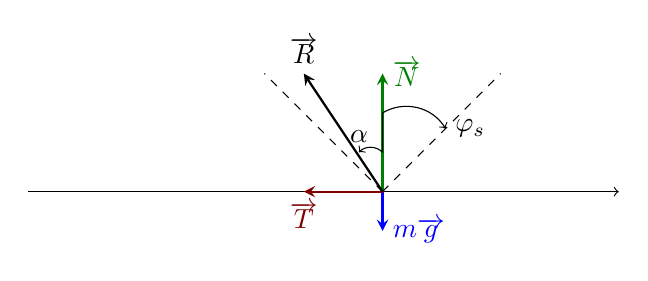
\begin{tikzpicture}[scale=1]  
                    % \helpgrid{3}{3}
                    \draw [->] (-4.5,-0.5) -- (3,-0.5) ;  
                    \coordinate (M) at (0,0); 
                    \draw [->,-stealth,thick,blue] (M) --++(0,-1) node [right] {$m\overrightarrow{g}$};   
                    \draw [->,-stealth,thick,green!50!black] (M)++(0,-0.5) --++(0,+1.5) node [right] {$\overrightarrow{N}$};
                    \draw [->,-stealth,thick,red!50!black] (M)++(0,-0.5) --++(-1,0) node [below] {$\overrightarrow{T}$};
                    \draw [->,-stealth,thick] (M)++(0,-0.5) --++(-1,1.5) node [above] {$\overrightarrow{R}$};
                    \draw[dashed] (M)++(0,-0.5) --++(-1.5,1.5);   
                    \draw[dashed] (M)++(0,-0.5) --++(1.5,1.5);
                    \draw[->] (M) to [bend right=45] (-0.3,0) node [above] {$\alpha$};
                    \draw[->] (M)--++(0,0.5) to [bend left=45] (0.8,0.3) node [right] {$\varphi_s$};
                \end{tikzpicture}
                \caption{Non glissement et cône de frottement statique.}    
                \label{fig:cone_frottement_statique}
            \end{figure}

            \begin{figure}
                \centering
                \tikzsetnextfilename{cone_frottement_dynamique}
                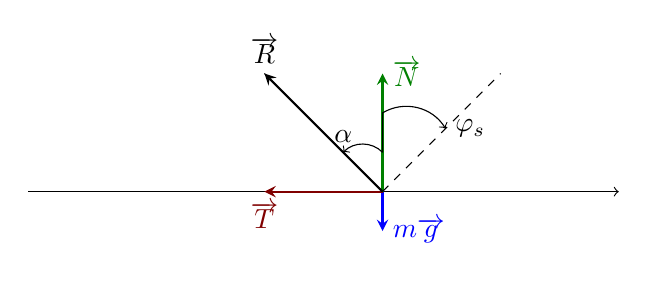
\begin{tikzpicture}[scale=1]  
                    % \helpgrid{3}{3}
                    \draw [->] (-4.5,-0.5) -- (3,-0.5) ;  
                    \coordinate (M) at (0,0); 
                    \draw [->,-stealth,thick,blue] (M) --++(0,-1) node [right] {$m\overrightarrow{g}$};   
                    \draw [->,-stealth,thick,green!50!black] (M)++(0,-0.5) --++(0,+1.5) node [right] {$\overrightarrow{N}$};
                    \draw [->,-stealth,thick,red!50!black] (M)++(0,-0.5) --++(-1.5,0) node [below] {$\overrightarrow{T}$};
                    \draw [->,-stealth,thick] (M)++(0,-0.5) --++(-1.5,1.5) node [above] {$\overrightarrow{R}$};
                    \draw[dashed] (M)++(0,-0.5) --++(-1.5,1.5);   
                    \draw[dashed] (M)++(0,-0.5) --++(1.5,1.5);
                    \draw[->] (M) to [bend right=45] (-0.5,0) node [above] {$\alpha$};
                    \draw[->] (M)--++(0,0.5) to [bend left=45] (0.8,0.3) node [right] {$\varphi_s$};
                \end{tikzpicture}
                \caption{Glissement et cône de frottement dynamique.}    
                \label{fig:cone_frottement_dynamique}
            \end{figure}

        \paragraph{Ordres de grandeur.} Le plus souvent, on a $f_s\approx f_d\coloneqq f$. On donne quelques valeurs de référence dans la Table~\ref{tab:odg_frottement_materiau}.

        \begin{table}
            \centering
            \begin{tabular}{l|c}
                \toprule
                Type de contact & $f$ \\ \midrule
                acier/acier & 0.2\\ \midrule
                acier/garniture de freins & 0.4\\ \midrule
                pneu/route sèche & 0.8\\ \midrule
                acier/bois & 0.5\\ \midrule
                bois/bois & 0.5\\ \midrule
                téflon/matière lisse & 0.04\\ \bottomrule
            \end{tabular}    
            \caption{Ordre de grandeur du coefficient de frottement pour quelques matériaux.}
            \label{tab:odg_frottement_materiau}
        \end{table}
    
    \subsection{Effet d'arc-boutement}
        
        Le modèle est présenté à la Figure~\ref{fig:modele_arcboutement}. On prend pour axe $(Ox)$ le plan incliné, orienté de gauche vers la droite, et l'axe $(Oy)$ est perpendiculaire à $(Ox)$ (orienté selon $\vec{N}$).

        \begin{figure}
            \centering
            \tikzsetnextfilename{modele_arcboutement}
            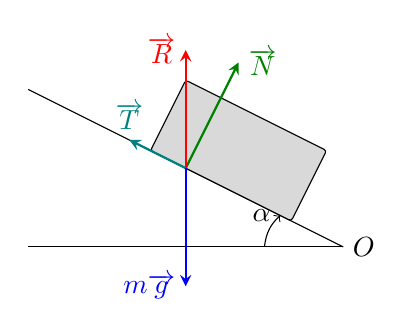
\begin{tikzpicture}[scale=1]  

                \coordinate (O) at (0,0); 
                \coordinate (A) at (-2,1); 
                \node at (O) [right] {$O$};
                \draw (O)--++(-4,0);
                \draw (O)--++(-4,2);

                \begin{scope}[rotate=atan((3-0)/(2-8))]
                    \draw  [rounded corners=1pt,fill=gray!30] ([shift={(-0.5,0)}]A) rectangle ++(2,1);
                    \draw [->,-stealth,thick,green!50!black] (A)--++(0,+1.5) node [right] {$\overrightarrow{N}$};
                    \draw [->,-stealth,thick,green!50!blue] (A)--++(-0.8,0) node [above] {$\overrightarrow{T}$};  
                \end{scope}

                \draw [->,-stealth,thick,blue] (A)--++(0,-1.5) node [left] {$m\overrightarrow{g}$};
                \draw [->,-stealth,thick,red] (A)--++(0,1.5) node [left] {$\overrightarrow{R}$};   
                \draw [->] (-1,0) to [bend left=20] (-0.8,0.4) node [left] {$\alpha$};
            \end{tikzpicture}
            \caption{Modèle d'arc-boutement.}
            \label{fig:modele_arcboutement}
        \end{figure}

        On se demande la condition sur $\alpha$ pour éviter tout glissement pour toute masse $m$. La condition de l'équilibre s'écrit $\vec{R}+m\vec{g}=\vec{0}$. En projetant sur $(Ox)$ puis $(Oy)$, on obtient
        \begin{equation*}
            \begin{aligned}
                mg\sin\alpha-T&=0,\\
                -mg\cos\alpha+N=0.
            \end{aligned}
        \end{equation*}
        Ainsi, on a $\frac{T}{N}=\tan\alpha$. On a donc non glissement si $T\leqslant f_s N$ ou bien $\alpha\leqslant\varphi_s$. C'est l'effet d'arc-boutement : pas de glissement quelque soit la charge.

        \paragraph{Condition de non-basculement.}

            Les équations en translation et rotation s'écrivent
            \begin{equation*}
                \begin{aligned}
                    \vec{R^{\text{ext}}}&=\vec{0}=\vec{R}+m\vec{g},\\
                    \vec{\mathcal{M}_{G}^{\text{ext}}}=\vec{0}=\vec{GG}\wedge m\vec{g}+\vec{GI}\wedge\vec{I},
                \end{aligned}
            \end{equation*}
            où $G$ est le centre de masse de la masse $m$, et $I$ est le point d'application de $\vec{R}$. Donc $\vec{GI}\parallel\vec{R}\parallel\vec{g}$. $I$ est donc à la vertical de $G$. On a non-basculement si $I$ reste sur la surface de contact : la limite du basculement est quand $I$ est sur l'arête. Ainsi, l'angle limite est tel que $\tan\alpha_{\text{lim}}=\frac{l}{h}$, où $l$ est la longueur de la masse et $h$ sa hauteur. Pour savoir s'il y a glissement ou basculement, il faut comparer $\frac{l}{h}$ et $f_s$.

    \subsection{Effet \og stick-slip\fg}

        C'est typiquement ce qu'il se passe en utilisant un archet enduit de colophane. Dans ce cas, on a $f_s\gg f_s$ (ici $f_d\approx0$). On considère le système présenté à la Figure~\ref{fig:archet_stick_slip}, la raideur du ressort est notée $k$, la masse de l'objet $m$.

        \begin{figure}
            \centering
            \tikzsetnextfilename{archet_stick_slip}
            \begin{tikzpicture}[scale=1]  

            \coordinate (O) at (0,0); 
            \node at (-3.6,0)[below] {O};
            
            \draw [->,-stealth,thick] (-3.6,0.35) -- (1,0.35) node [below]{$z$};
            
            %ressort   
            \begin{scope}[shift=({0,0})]     

            \begin{scope}[scale=0.75,shift=({-4.78,0.5}),rotate around={90:(0,0)}]
            %bloc qui tient le ressort
                \draw[thick,gray] (0,0) -- (0,-0.3); 
                \fill [pattern=north east lines] (-0.5,0) rectangle (0.5,0.3); 
                \draw[thick](-0.5,0)--(0.5,0);
                %fin ressort       
            \end{scope}	

            \draw [ressort,decorate,decoration={coil,aspect=0.6,segment length=5mm,amplitude=3mm}] (-3.375,0.36)--++(3,0) ;
            \draw[rounded corners=1pt,fill=gray!30] (-0.5,0.35) rectangle++ (0.5,0.5) node [midway, shift=({0,0.05})] {$\centerdot$};  

            \draw [->,green!50!black,very thick] (-0.25,0.35)--++(1,0) node [below] {$\overrightarrow{T}$};
            \draw [->,red!50!black,very thick] (-0.5,0.57)--++(-0.5,0) node [above] {$\vec{f}_{el}$};
            \end{scope}

        \end{tikzpicture}
        \caption[Effet \og stick-slip\fg.]{Effet \og stick-slip\fg. L'axe $(Ox)$ est un tapis roulant vers la droite de vitesse $\vec{v}=V\vec{u_x}$}
        \label{fig:archet_stick_slip}
        \end{figure}

        \begin{itemize}
            \item \underline{Phase 1} : non glissement sur $[0,t_1]$. On a 
            \begin{equation*}
                m\ddot{x}=0=-kx+T,
            \end{equation*}
            doù $x(t)=Vt$. La fin de la phase 1 à $t_1$ a lieu quand $T=f_s N$. On a $T(t_1)=kx(t_1)=kVt_1$ et $N=mg$. Ainsi,
            \begin{equation*}
                f_1=f_s\frac{mg}{kV}=\frac{f_s g}{\omega_{0}^{2}V},
            \end{equation*}
            avec $\omega_{0}^{2}=\frac{k}{m}$.

            \item \underline{Phase 2} : on a glissement. $f_d\approx0$ donc il y a glissement sans frottement. Ainsi,
            \item \begin{equation*}
                m\ddot{x}=-kx+0,
            \end{equation*}
            d'où $\ddot{x}+\omega_{0}^{2}x=0$. Alors $x(t\geqslant t_1)=A\cos\left(\omega_0(t-t_1)+\alpha\right)$. La condition initiale est en $t=t_1$ : on a $x(t_1)=Vt_1=\frac{f_s g}{\omega_{0}^{2}}=A\cos\alpha$, et $\dot{x}(t_1)=V=-A\omega_0\sin\alpha$. Alors
            \begin{equation*}
                \tan\alpha=-\frac{\omega_0 V}{f_s g},\qquad A^{2}=\left(\frac{f_s g}{\omega_{0}^{2}}\right)^{2}+\left(\frac{V}{\omega_0}\right)^{2}.
            \end{equation*}

            On a fin du glissement à $t=t_2$, c'est-à-dire $Vg(t_2)=0$, d'où $\dot{x}(t_2)=V$. Alors
            \begin{equation*}
                -A\omega_0\sin\left(\omega_0(t_2-t_1)+\alpha\right)=V=-A\omega_0\sin\alpha,
            \end{equation*}
            puis
            \begin{equation*}
                \sin\left(\omega_0(t_2-t_1)+\alpha\right)=\sin\alpha,
            \end{equation*}
            d'où $\omega_0(t_2-t_1)+\alpha=\pi-\alpha$, ce qui donne enfin
            \begin{equation*}
                t_2-t_1=\frac{\pi}{\omega_0}-\frac{2\alpha}{\omega_0}.
            \end{equation*}

            \item \underline{Phase 3} : non glissement sur $[t_2,t_3]$, on a 
            \begin{equation*}
                \dot{x}(t_2\leqslant t\leqslant t_3)=V,
            \end{equation*}
            d'où $x(t_2\leqslant t_\leqslant t_3)=V(t-t_2)+K$. La condition initiale donne
            \begin{equation*}
                K=x(t_2)=A\cos\left(\omega_0(t_2-t_1)+\alpha\right)=A\cos\left(\pi-\alpha\right)=-A\cos\alpha.
            \end{equation*}
            Ainsi,
            \begin{equation*}
                x(t_2\leqslant t\leqslant t_3)=V(t-t_2)-A\cos\alpha.
            \end{equation*}
            Le fin de la phase 3 a lieu en $t_3$ quand $T(t_3)=f_s N=f_s mg$. Or $m\ddot{x}=0=T-kx$, donc $kx(t_3)=f_s mg$. Donc
            \begin{equation*}
                kV(t_3-t_2)-k\frac{f_s g}{\omega_0^{2}}=f_s mg.
            \end{equation*}
            Donc 
            \begin{equation*}
                t_3-t_2=2\frac{f_s g}{\omega_0^{2}V}.
            \end{equation*}
        \end{itemize}





